\documentclass[12pt,a4paper,oneside]{book}

\makeatletter
\newcommand\thefontsize[1]{{}}
\makeatother
\usepackage[utf8]{inputenc}
\usepackage{enumitem}
\usepackage{varwidth}
\usepackage{graphicx}
\usepackage{float}
\usepackage{caption}

\usepackage[top=2.5cm, bottom=3cm, left=2.5cm, right=2.5cm]{geometry}
\usepackage[utf8]{inputenc}
\usepackage[titletoc,title]{appendix}
\usepackage[linewidth=1pt]{mdframed}
\usepackage{framed}
\usepackage{listings}
\usepackage{smartdiagram}
\usepackage{smartdiagram}
\usepackage{varwidth}
\usepackage{amsmath}
\usesmartdiagramlibrary{additions}
\lstdefinestyle{customc}{
	belowcaptionskip=1\baselineskip,
	breaklines=true,
	frame=L,
	xleftmargin=\parindent,
	language=C,
	showstringspaces=false,
	basicstyle=\footnotesize\ttfamily,
	keywordstyle=\bfseries\color{green!40!black},
	commentstyle=\itshape\color{purple!40!black},
	identifierstyle=\color{blue},
	stringstyle=\color{orange},
}

\lstdefinestyle{customasm}{
	belowcaptionskip=1\baselineskip,
	frame=L,
	xleftmargin=\parindent,
	language=[x86masm]Assembler,
	basicstyle=\footnotesize\ttfamily,
	commentstyle=\itshape\color{purple!40!black},
}

\lstset{escapechar=@,style=customc}

\lstset{
	literate=%
	{à}{{\'a}}1
	{í}{{\'i}}1
	{é}{{\'e}}1
	{è}{{\`e}}1
	{ý}{{\'y}}1
	{ú}{{\'u}}1
	{ó}{{\'o}}1
	{ě}{{\v{e}}}1
	{š}{{\v{s}}}1
	{č}{{\v{c}}}1
	{ř}{{\v{r}}}1
	{ž}{{\v{z}}}1
	{ď}{{\v{d}}}1
	{ť}{{\v{t}}}1
	{ň}{{\v{n}}}1
	{ů}{{\r{u}}}1
	{Á}{{\'A}}1
	{Í}{{\'I}}1
	{É}{{\'E}}1
	{Ý}{{\'Y}}1
	{Ú}{{\'U}}1
	{Ó}{{\'O}}1
	{Ě}{{\v{E}}}1
	{Š}{{\v{S}}}1
	{Č}{{\v{C}}}1
	{Ř}{{\v{R}}}1
	{Ž}{{\v{Z}}}1
	{Ď}{{\v{D}}}1
	{Ť}{{\v{T}}}1
	{Ň}{{\v{N}}}1
	{Ů}{{\r{U}}}1
}

\begin{document}

	\def\reportnumber{}
	\def\reporttitle{Inférence logique et propagation graphique }
	%----------------------------------------------------------------------------------------
%	TITLE PAGE
%----------------------------------------------------------------------------------------

\begin{titlepage} % Suppresses displaying the page number on the title page and the subsequent page counts as page 1
	\newcommand{\HRule}{\rule{\linewidth}{0.5mm}} % Defines a new command for horizontal lines, change thickness here
	
	\center % Centre everything on the page
	
	%------------------------------------------------
	%	Headings
	%------------------------------------------------
	
	\baselineskip=2\baselineskip 
	\textsc{\LARGE Université des Sciences et de la Technologie Houari Boumediene}%\\[1cm] % Main heading such as the name of your university/college

	%------------------------------------------------
	%	Logo
	%------------------------------------------------
	
	%\vfill\vfill
	\vfill
	
\includegraphics[width=0.3\textwidth]{USTHB_Logo.png}\\[1cm] % Include a department/university logo - this will require the graphicx package
	 
	%----------------------------------------------------------------------------------------
	
	\textsc{\Large RCR2 }\\[0.5cm] % Major heading such as course name
	%\textsc{\large Minor Heading}\\[0.5cm] % Minor heading such as course title
	
	%------------------------------------------------
	%	Title
	%------------------------------------------------
	
	\HRule\\[0.4cm]
	\baselineskip=1.2\baselineskip 
	{\huge\bfseries Rapport du TP\text  \reportnumber \\ \reporttitle}\\[0.4cm] % Title of your document
	
	\HRule\\[1.5cm]
	
	%------------------------------------------------
	%	Author(s)
	%------------------------------------------------
	
	\begin{minipage}{0.4\textwidth}
		\begin{flushleft}
			\large
			\textit{Rédaction:}\\
			MOULAI \textsc{Hassina Safaa}\\ % Your name
			Matricule : 201400007564\\ 
			
			HOUACINE \textsc{Naila Aziza}\\ % Your name
			Matricule : 201400007594\\ 
			
			M2 SII Groupe:3\\
			
		\end{flushleft}
	\end{minipage}
	~
	\begin{minipage}{0.4\textwidth}
		\begin{flushright}
			\large
			\textit{Professeur}\\
			Mme. Hedjazi Badiaa  % Supervisor's name
		\end{flushright}
	\end{minipage}
	
	%------------------------------------------------
	%	Date
	%------------------------------------------------
	
	\vfill\vfill\vfill % Position the date 3/4 down the remaining page
	
	{\large\today} % Date, change the \today to a set date if you want to be precise
	
	
	\vfill % Push the date up 1/4 of the remaining page
	
\end{titlepage}
	
	\tableofcontents

	\listoffigures

	
	\chapter{Introduction }
	Nous avons précedemment (dans le module RC1) manipulé les notion d'inférence logique avec Max-Sat, mais plusieurs autre méthodes existe dont les méthodes graphiques.
	
	Le présent TP est orienté théorie des possibilités, celui-ci pouvant être modélisé aussi bien graphiquement que par une représentation MAX Weighted SAT, nous avons pour but de tester les deux méthodes sur différents problèmes c'est à dire représenté nous forme de polytree, graph multiconnected et graph simply connected.\\
	
	Pour cela deux outils largement utilisé dans ce domaine ont été mis à notre disposition, Il s'agit de la \textbf{PNT} de \textbf{Matlab} et l'outil \textbf{cygwin} sous Windows.\\

Ainsi nous allons grâce à ces outils comparer les temps d'inférence logique avec les temps de propagation de la méthode graphique afin de comprendre les avantages et inconvenants de chacun, et de savoir sur quelle base choisir la méthode d'inférence du degrés de possibilité la plus adéquate.
	
	
	\chapter{Réalisation}
	\section{L'outil cygwin}
	Cygwin est une collection de logiciels libres à l'origine développés par Cygnus Solutions permettant à différentes versions de Windows de Microsoft d'émuler un système Unix. Il vise principalement l'adaptation à Windows de logiciels qui fonctionnent sur des systèmes POSIX (tels que les systèmes GNU/Linux, BSD, et Unix). Cygwin simule un environnement Unix sous Windows, rendant possible l'exécution de ces logiciels après une simple compilation.[1] 
	
	\section{Étape 1:}
	\subsection{Utilisation du prod1vid.m}
	 principalement prod1vid construit un réseau causal probabiliste basé sur le produit tel que les connexions entre les nœuds sont aléatoires , ainsi que les valeurs initiales attribués à la variable d'intérêt et l'évidence .
	 Pour exécuter le programme il faut:
	 \begin{itemize}
	 	\item sur Matlab taper : prod1vid
	 	
	 \end{itemize}
	 ce que le programme offre en sortie est environnement ou on peut voir toutes les variables et le graphe (matrice) crée.
	 on peut alors afficher :
	 
	 \begin{itemize}
	 	\item la variable d'intérêt sachant l'évidence
	 	\item temps de la propagation
	 	\item type de graphe (multi-connected (multi-connectés) ou polytree (polyarbre))
	 \end{itemize}
	 \subsubsection{Fonctionnement du programme}
	 Aprés avoir étudier le programme on a pu résumer son fonctionnement dans les étapes qui suivent :
	 \begin{enumerate}
	 	\item Initialisation du nombre de parents max globale et nombre de noeuds du graphe à construire
	 	\item Création de liens de façon aléatoire entre les noeuds.
	 	\item Utilisation de processus de fixation après la création aléatoire afin d'éviter les noeuds isolés et sous graphes isolés ( les inconvénients de l'aléatoire)
	 	\item Prise de considération des domaines des variables (représentés par les noeuds)
	 	cas binaire etc ...
	 	\item Génération de la distribution aléatoire initiale du graphe crée (de possibilité initiales).
	 	\item génération aléatoire d'une évidence  : une évidence est une information nouvelle qui viens et à qui on aimerait calculer l'influence qu'elle aura sur la variable d'intérêt(évidente est comme une condition ).
	 	\item Détermination si le graphe est polytree ou multi-connected
	 	\item Lancement de la propagation ( algorithme de propagation)
	 	
	 	
	 \end{enumerate}
	 
	 Concernant \textbf{Prodevid2} c'est le mème fonctionnement à part qu'on a droit à deux évidences donc deux informations vont influer notre réseau , en théorie  on peut penser que la propagation des deux évidences prendra plus de temps que celle d'une seule , on testera ce cas dans ce qui suit .
	 
	
	\subsection{Réglage de paramètres}
	\subsubsection{Jeu de test}
	On a choisi de fixer le nombre de noeuds à :10
	
	et le nombre de parent max à :2 
	
	ce qui est censé nous donnée un polytree .
	\subsubsection{Code}
	
    	\begin{figure}[h]
		\centering
		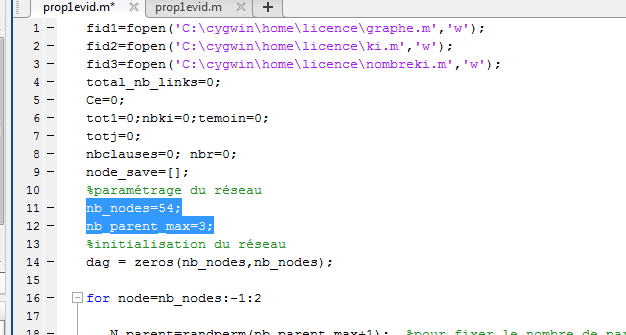
\includegraphics[scale=0.7]{screens/prodevid1code.png}
		\captionof{figure}{Le changement des nb noeuds ainsi que nb parents max dans le code prod1evid.m}\label{labelname}%
		\end{figure}
	
	On a choisi de fixer \textbf{le nombre de nœuds à : 54}
	
	et \textbf{le nombre de parents max à :3 }
	
   \paragraph{Remarque}
   Dans le code fourni Pour avoir le nombre de parents d'un nœud , le programme tire aléatoirement un nombre entre \textbf{[1,nbparentsmax+1]} donc concrètement  le nombre de parents max est de 4 et non de 3  voir code:prod1evid.m.
   
	\subsubsection{Affichage}
	le résultat était le suivant :
	
	
	\begin{frame}{}
		\centering
		\begin{minipage}[H]{0.5\linewidth}
			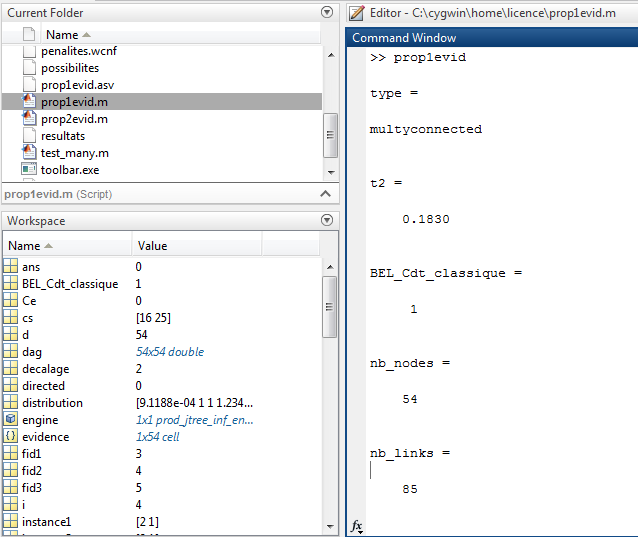
\includegraphics[width=1\textwidth]{screens/prodevid1affichge.png}%
			\captionof{figure}{Une seule evidence}\label{labelname}%
		\end{minipage}
		\hspace{0.5cm}
		\begin{minipage}[H]{0.5\linewidth}
			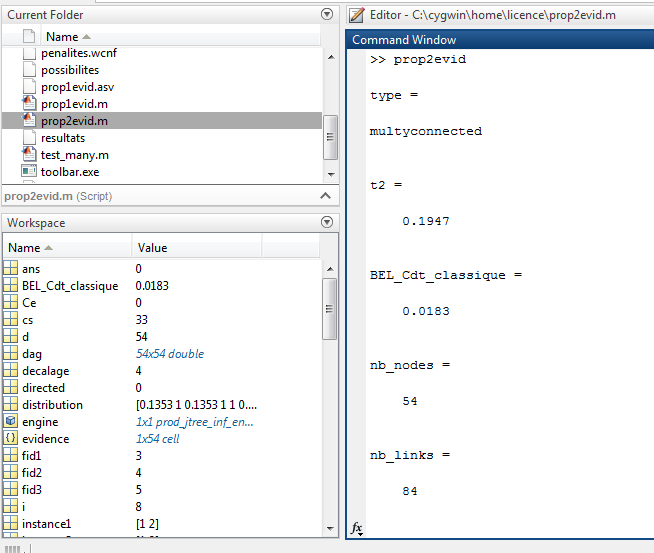
\includegraphics[width=1\textwidth]{screens/prodevid2affichage.png}%
			\captionof{figure}{Deux evidences}\label{labelname}%
		\end{minipage}
	\end{frame}

		\begin{center}
			\begin{tabular}{ | l || c | c | }
				\hline
				\textbf{nombre d'évidence} & 1 &  2\\
				\hline
				\textbf{temps de propagation} & 0.18 secondes & 0.19 secondes\% \\
				\hline
				\textbf{Bel variable d'intérêt} & 1 & 0.018 \\
				\hline
			\end{tabular}
		\end{center}

		
	\subsubsection{Observation}
    	Comme on a pu le deviner la propagation prend plus de temps avec deux évidences qu'avec une seule , car le calcul des nouvelles distributions de possibilités conditionnelles est plus complexe avec deux informations (deux conditions) qui arrivent qu'avec une seule (une seule condition) .
	
	\newpage
	
	\section{Étape 2}
	\subsection{Explication  }
      Dans cette étape il nous ai demandé d'utiliser deux programmes exécutables
      à fin de passer d'une modélisation graphique avec des algorithmes de propagation à une une représentation logique en clauses (max sat weighted ) en utilisant le processus d'inférence.
            Prodevid1 donne en sortie un graphe ( matrice en matlab) qui modélise le graphe crée
            \begin{figure}[H]
            	\centering
            	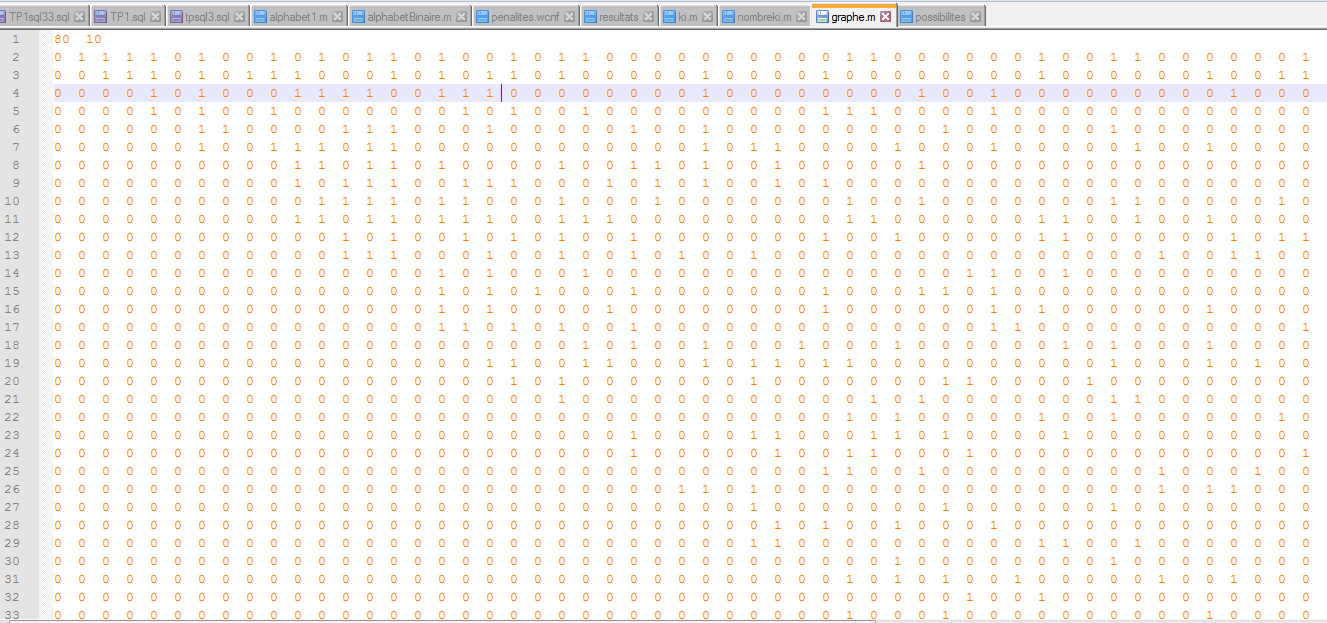
\includegraphics[scale=0.7]{screens/etape2graph.png}
            	\captionof{figure}{exemple d'un graphe en sortie à l'éxecution de  prod1evid.m avec noeuds=80 et parents =10}\label{labelname}%
            	
            \end{figure}
            \begin{figure}[H]
            	\centering
            	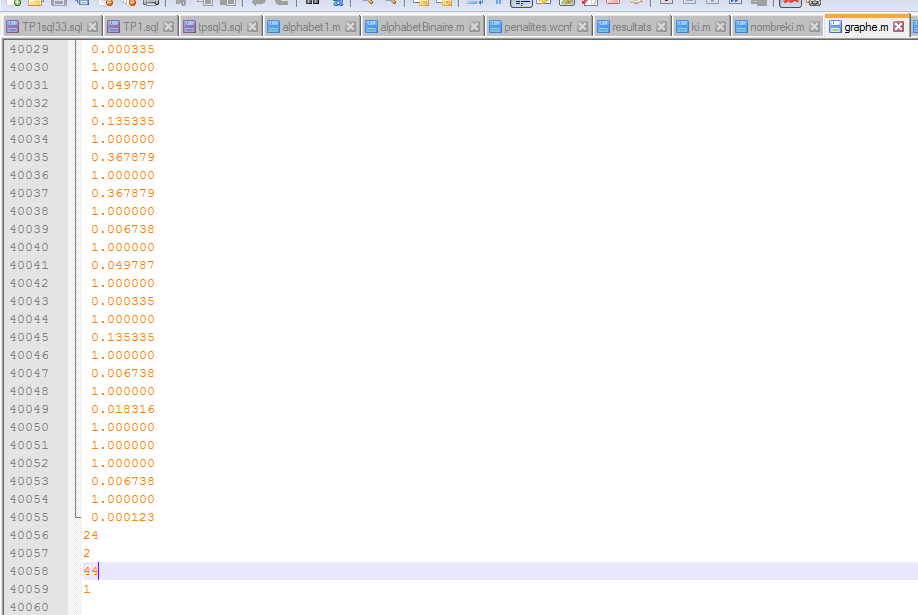
\includegraphics[scale=0.7]{screens/etape2graph2.png}
            	\captionof{figure}{exemple d'un graphe en sortie à l'éxecution de  prod1evid.m avec noeuds=80 et parents =10}\label{labelname}%
            \end{figure}
      
      Tout d'abord on reprend l'exemple vu dans l'étape 1 avec un nombre de noeuds à 54 et nombre de parents max à 4 puis il faudra faire :
      \begin{itemize}
      	\item Se placer dans le dossier licence sous terminal de cygwin .
      	\item Exécuter le prod1evid sous matlab
      	\item Exécuter le ./passage.exe qui convertit les graph.m en clauses (maxSat)
      	\item Lancement du processus d'inférence on aura le temps de l'inférence en MICRO SECONDES.
      	\item Affichage du résultat avec la commande : cat résultats
      \end{itemize}
      
      \subsubsection{Affichage}
      
      
      
      	
      		\begin{figure}[H]
      				\centering
      			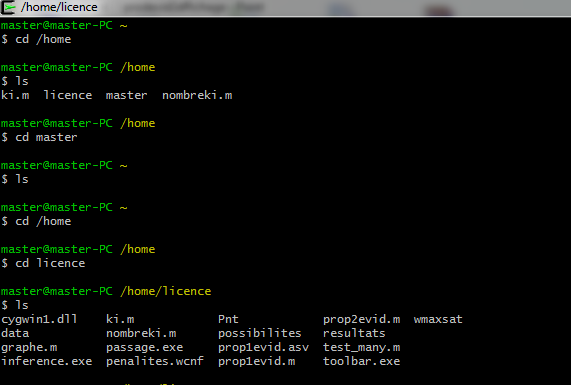
\includegraphics[scale=1]{screens/etape2terminal.png}%
      			\captionof{figure}{Les commandes necessaires pour lancer l'inference}\label{labelname}%
      		\end{figure}
      		
      		\begin{figure}[H]
      				\centering
      			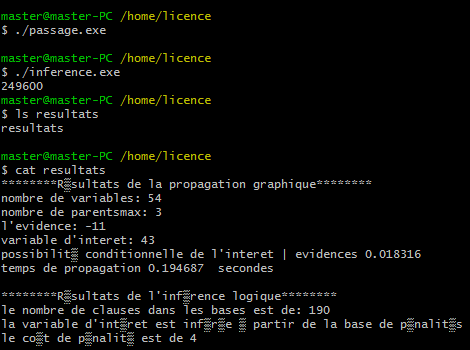
\includegraphics[scale=1.1]{screens/etape2.png}%
      			\captionof{figure}{Lancement de passage et inference }\label{labelname}%
      		\end{figure}
        
        
        \subsubsection{Observation}
        on remarque dans notre cas on à affaire a un réseau multi-connected on a remarqué que la propagation prenait presque autant de temps que l'inférence , on peut expliquer ça par le fait qu'on manipule des graphes où le nombres de noeuds et connexions n'est pas conséquent par contre dans le cas ou le nombre de noeuds était 80 et parents = 10 la propagation avait pris beaucoup plus de temps  voir l'etape 3 comparé à l'inférence qui fait appel à un solver max sat .

       
    \section{Étape 3}
    \subsection{Génération automatique aléatoire des Graphes}
    \subsubsection{Génération des Polytree}
    Un \textbf{polytree} est un graphe ayant les particularités suivantes: c'est un graphe orienté (les arcs reliant les noeuds sont orienté parent $\rightarrow$ fils),connexe (pas de noeuds ou sous arbre libre), acyclique (ne contient pas de cycle/ boucle), et enfin simplement connecté.\\
    
    Ainsi afin d'obtenir des polytree, nous avons limité le nombre maximum de parent à 1 seul parent.
    
    Par contre, pour ce qui est du nombre de noeuds nous avons le choix, mais nous nous sommes limité aux testes montrés dans le tableau récapitulatif plus bas.
    
 
    
    \subsubsection{Génération des Multiconnected}
    On parle graphes \textbf{Multiconnected} lorsque nous avons un graphe orienté (les arcs reliant les noeuds sont orienté parent $\rightarrow$ fils),connexe (pas de noeuds ou sous arbre libre), acyclique (ne contient pas de cycle/ boucle), et enfin à connections multiple de ses nœuds.\\
    
    Pour obtenir cette catégorie de graphe nous pris des nombres de parents supérieur à 1 , et même de l'ordre de 7 à 10 parents par noeuds, toujours en faisant varier le nombre de noeuds, afin de diversifier les résultats et explorer plus de combinaison.
    
    \subsubsection{Génération des Simply connected}
    la notion de simple connexité raffine celle de connexité : là où un espace connexe est simplement "d'un seul tenant", un espace simplement connexe est de plus sans "trou" ni "poignée" mais nous parlant toujours de graph sans boucles.[2]\\
    
     De manière analogue que pour les deux type de graphes précédents nous avons généré ce type de graphe selon le nombre de noeuds et de parent et obtenu les résultats regroupés dans la section "résultats".
    
    \newpage
    
    \section{Résultats}
    Suite à maintes expérimentations et testes avec les différentes configurations précédentes, nous avons résumé quelques résultats dans le tableau suivant: 
\begin{center}
\begin{tabular}{|l||c|c|c|}
	\hline
	\textbf{NbrNœuds/NbrParents} &	\textbf{Temps Propagation} & \textbf{Temps Inférence} &  \textbf{Degrés Possibilité}
	\\
	\hline
	

		
	%\newline
	\textbf{25 Nœuds / 1 Parents} & 0.156598 sec & 0.171601 sec  & 0.049787
	\\
	\hline
	
	%\newline
	\textbf{50 Nœuds / 1 Parents} & 0.282039 sec & 0.218400 sec  & 1
	\\
	\hline
	
	%\newline
	\textbf{15 Nœuds / 3 Parents} & 0.052538 sec & 0.156000 sec  & 0.049787
	\\
	\hline
	
	%\newline
	\textbf{25 Nœuds / 4 Parents} &  0.081438 sec & 0.156000 sec  & 1
	\\
	\hline
	
	%\newline
	\textbf{25 Nœuds / 7 Parents} & 0.078056 sec & 0.249600 sec  & 1
	\\
	\hline
	
	%\newline
	\textbf{25 Nœuds / 10 Parents} & 0.55983 sec & 0.315625 sec  & 0.018316
	\\
	\hline
	
	%\newline
	\textbf{40 Nœuds / 10 Parents} &  14.1780 sec & 0.50927 sec & 0.36788
	\\
	\hline
	
	
	%\newline
	\textbf{30 Nœuds / 7 Parents} &  0.094228 sec & 0.218401 sec & 1
	\\
	\hline
	
	%\newline
	\textbf{30 Nœuds / 1 Parent} &  0.196302 sec & 0.187200 sec & 0.018316
	\\
	\hline
	
	%\newline
	\textbf{80 Nœuds / 10 Parents} & pc stopped & pc stopped   & pc stopped
	\\
	\hline
	
	%\newline



\end{tabular} 
\end{center}
Quelques résultats sont mis dans l'annexe sous forme de capture d'ecran.
    
    \section{Observation pour chaque type }
    \subsection{Observation pour les Polytree}
    Comme le montre les résultats précédemment obtenus, les polytree sont déja très rapide en temps de construction, puis nous remarquons que ce soit par la méthode graphique \textbf{(Propagation)} ou la méthode logique \textbf{(Inférence)} les degrés de possibilité sont donné très rapidement, même que pour certains cas la méthode graphique est très légèrement plus rapide
    
  
    
    
    \subsection{Observation pour les Multiconnected}
    D'après les résultats produits suite aux nombreuses expérimentations que nous avons effectué, nous somme en mesure de souligner la rapidité de la méthode d'inférence logique (basé maw weighted sat) comparé à la méthode graphique (propagation), tel que pour de grandes instances / graphe multiconnectés (beaucoup de noeuds et beaucoup d'arcs) la méthode d'inférence logique reste raisonnablement rapide, légèrement plus lente que pour les polytree, contrairement à la méthode graphique de propagation qui voit le temps de propagation croitre de l'ordre de 10 aine, jusqu'à ne plus être exécutable sur nos machine comme pour (80 noeuds et 10 parents).
    

    
    \subsection{Observation pour les Simply connected}
    En vu des résultats des expérimentations sur ce type de graphe nous avons constaté que le temps de propagation via la méthode graphique est plus rapide que le temps d'inférence de la méthode logique , bien que les deux reste inférieur à 1 second.
    
    \newpage
    \chapter{Conclusion et comparaison}
    Suite aux expérimentation effectuées avec les deux techniques misent à notre disposition lors de ce Tp, nous pouvons constater que la méthode d'inférence logique est bien plus rapide et efficace que la méthode graphique de propagation.\\
    
    Car bien que les méthodes graphiques soient plus parlantes et lisible pour l'humain, leurs complexité n'en est pas pour autant bonne, car en plus du temps de propagation très lent pour les grandes instances de problème (multiconnected), la méthode de propagation nécessite aussi la construction de l'arbre de jonction qui prends elle aussi un temps non négligeable.\\
    
    Ainsi à la limite pour les polyarbe nous pouvant utiliser les deux méthodes car bien que la méthode graphique soit légèrement plus rapide que celle d'inférence logique, les deux méthodes donne le résultats très rapidement, d'ailleurs la méthode graphique ne nécessite pas dans ce cas là la construction de l'arbre de jonction.
      

\newpage
\chapter*{Bibliographie}
\textbf{ }\\

[1] : https://fr.wikipedia.org/wiki/Cygwin
\textbf{ }\\

[2] : https://fr.wikipedia.org/wiki/Connexit\%C3\%A9\_simple

\chapter*{ANNEXE}
\begin{figure}[H]
	\centering
	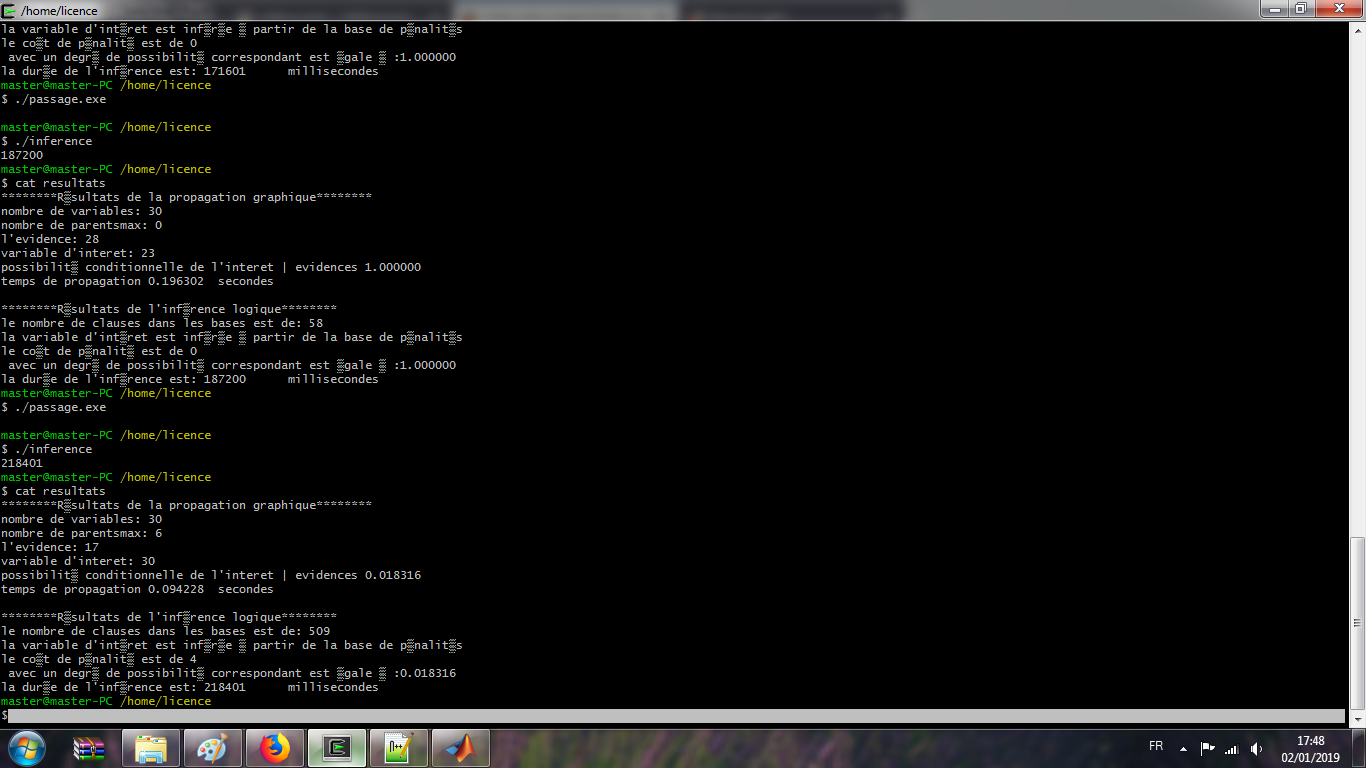
\includegraphics[scale=0.4]{screens/multiconnected.png}%
	\captionof{figure}{Expérimentation 1 }\label{labelname}%
\end{figure}

\begin{figure}[H]
	\centering
	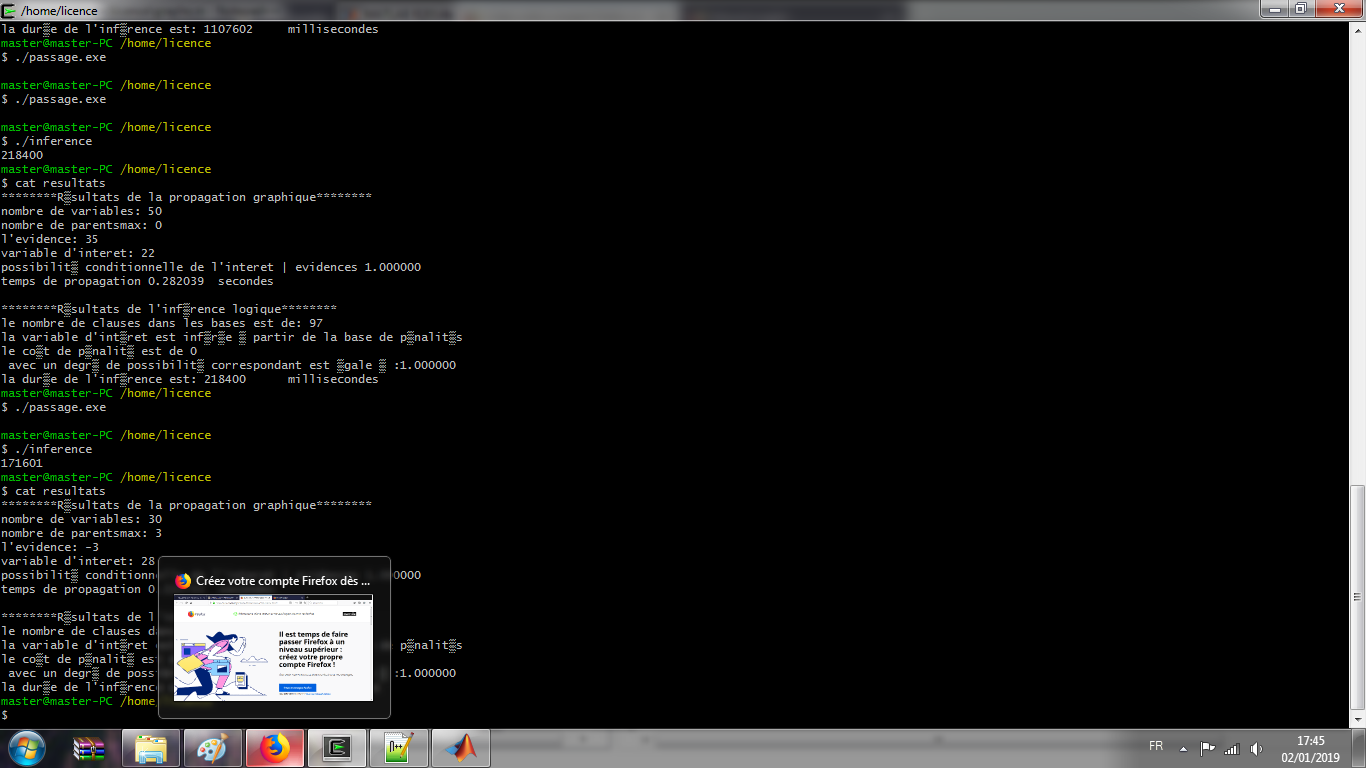
\includegraphics[scale=0.4]{screens/polytree.png}%
	\captionof{figure}{Expérimentation 2 }\label{labelname}%
\end{figure}

\begin{figure}[H]
	\centering
	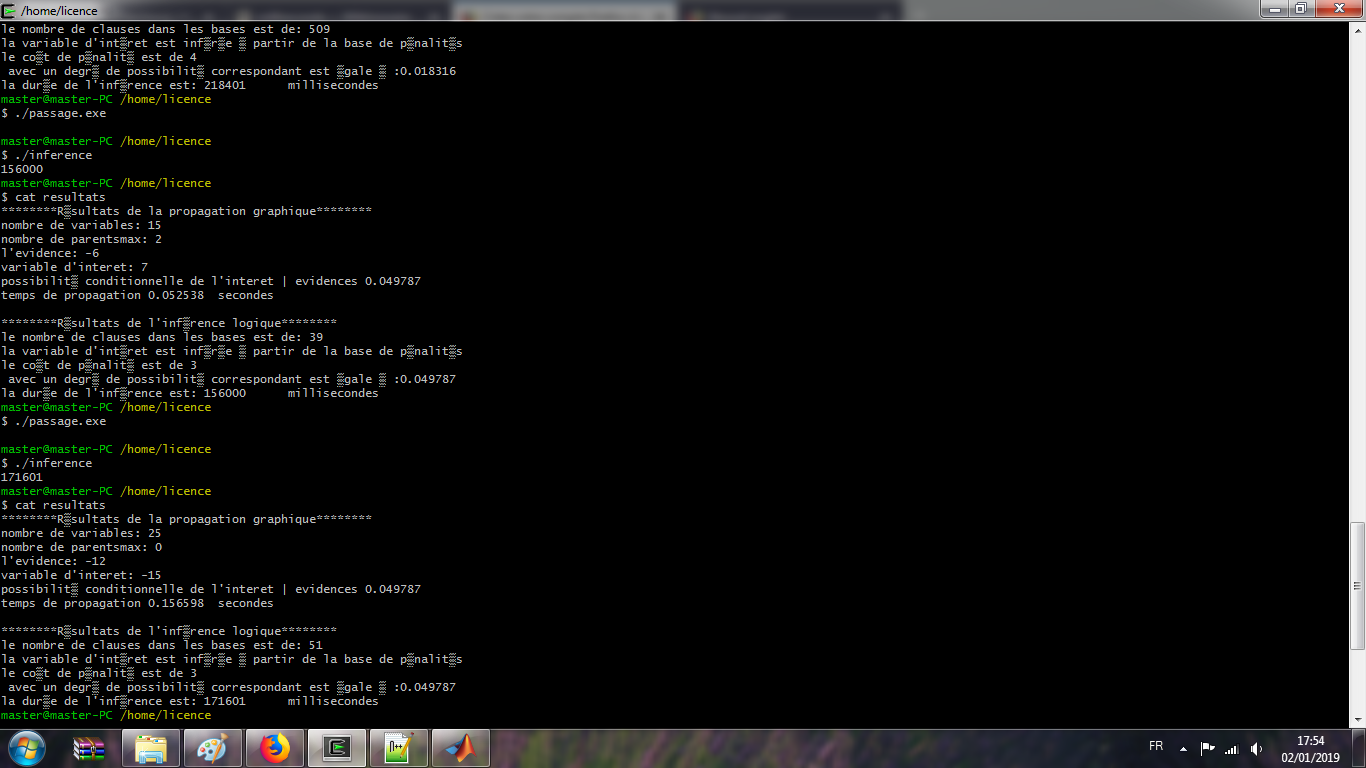
\includegraphics[scale=0.4]{screens/25_0.png}%
	\captionof{figure}{Expérimentation 3}\label{labelname}%
\end{figure}

\begin{figure}[H]
	\centering
	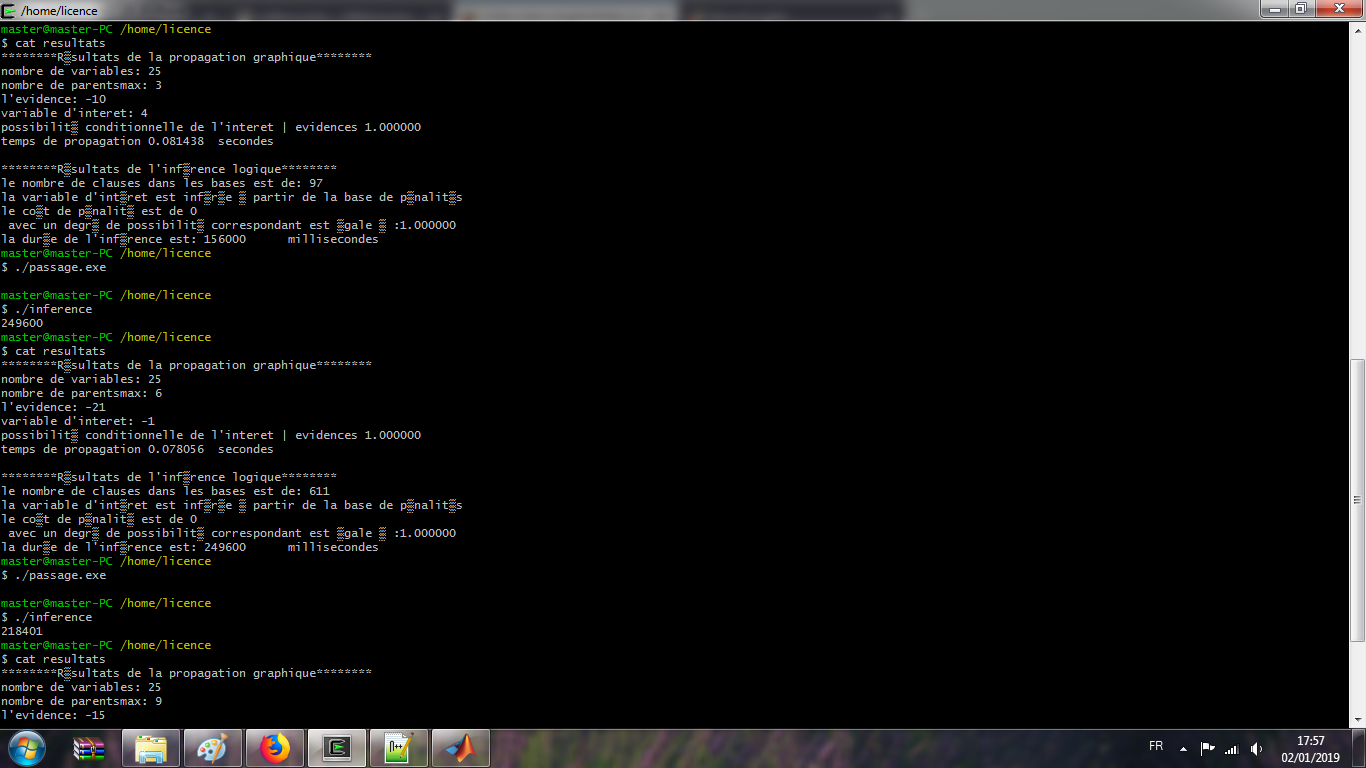
\includegraphics[scale=0.4]{screens/25_3_6.png}%
	\captionof{figure}{Expérimentation 4 }\label{labelname}%
\end{figure}






\end{document}